\section{Project Objective}
\label{sec:objective}

The objective of this thesis is to compile a logical OpenQASM circuit into a physical circuit on Pasqal's neutral atom quantum computer. 
This is achievable in four steps, the first is to parse the QASM code to retrieve the number of qubits 
used and which gates are applied to them. Once the code has been parsed, the qubits are mapped into a register that satisfies the constraints imposed by the multi-qubit gates. Following the creation of the register 
the gates can be translated into adequate optical pulses. 
Finally, the compiled quantum circuit can be tested through simulation, or on a real quantum device if available.
\begin{figure}[H]
    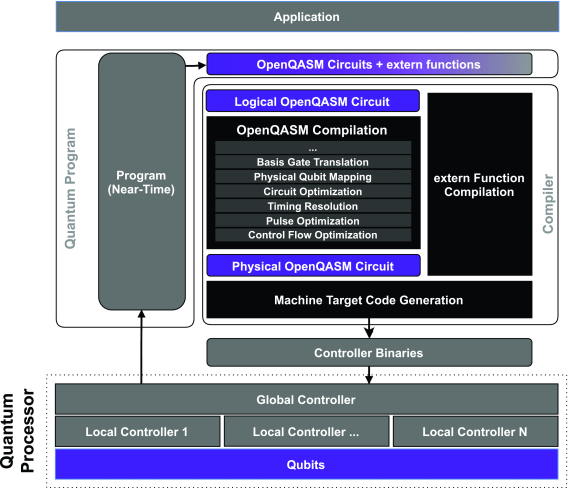
\includegraphics[scale=16]{./Images/compilation_chart.jpg}
    \caption{Flowchart detailing compilation steps for OpenQASM on a generalised quantum computer. Note that the optimization steps in the OpenQASM compilation are not in the scope of this project.} 
    \label{fig:compchart}
  \end{figure}